
% \figninepanelwidth is the final size; no outer scaling is applied.
\begin{figure}[!ht]
    \centering
    \begingroup
    \newlength{\figninepanelwidth}
    \newlength{\figninelegendunit}
    \setlength{\figninepanelwidth}{1.55in}
    \setlength{\figninelegendunit}{\dimexpr\figninepanelwidth*10/52\relax}

    
    \definecolor{fignineTKE0}{RGB}{4,41,91}
    \definecolor{fignineTKE1}{RGB}{27,59,111}
    \definecolor{fignineTKE2}{RGB}{64,76,108}
    \definecolor{fignineTKE3}{RGB}{89,95,109}
    \definecolor{fignineTKE4}{RGB}{111,113,115}
    \definecolor{fignineTKE5}{RGB}{134,131,120}
    \definecolor{fignineTKE6}{RGB}{159,150,116}
    \definecolor{fignineTKE7}{RGB}{184,171,108}
    \definecolor{fignineTKE8}{RGB}{212,193,92}
    \definecolor{fignineTKE9}{RGB}{239,217,69}

    \newcommand{\figninelegendbar}{%
        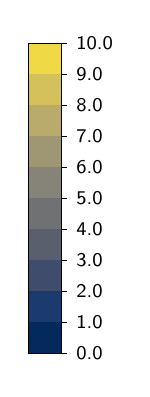
\begin{tikzpicture}[baseline=0pt,x=1cm,y=\figninelegendunit]
            \fill[fignineTKE0] (0,0.00) rectangle (0.42,0.52);
            \fill[fignineTKE1] (0,0.52) rectangle (0.42,1.04);
            \fill[fignineTKE2] (0,1.04) rectangle (0.42,1.56);
            \fill[fignineTKE3] (0,1.56) rectangle (0.42,2.08);
            \fill[fignineTKE4] (0,2.08) rectangle (0.42,2.60);
            \fill[fignineTKE5] (0,2.60) rectangle (0.42,3.12);
            \fill[fignineTKE6] (0,3.12) rectangle (0.42,3.64);
            \fill[fignineTKE7] (0,3.64) rectangle (0.42,4.16);
            \fill[fignineTKE8] (0,4.16) rectangle (0.42,4.68);
            \fill[fignineTKE9] (0,4.68) rectangle (0.42,5.20);
            \draw[line width=0.35pt] (0,0) rectangle (0.42,5.20);
            \foreach \y/\ticklabel in {
                0.00/0.0,0.52/1.0,1.04/2.0,1.56/3.0,2.08/4.0,
                2.60/5.0,3.12/6.0,3.64/7.0,4.16/8.0,4.68/9.0,5.20/10.0}
                {\draw[line width=0.3pt] (0.42,\y) -- (0.49,\y)
                 node[anchor=west,font=\sffamily\fontsize{7.5}{8}\selectfont]
                 {\ticklabel};}
        \end{tikzpicture}%
    }

    \newcommand{\figninepanellabel}[2]{%
        {\sffamily\bfseries\fontsize{8.5}{9.5}\selectfont
         (#1) $h_d/l_d=#2$}%
    }

    \begin{tabular}[c]{@{}l@{\hspace{0.10in}}c@{\hspace{0.05in}}c@{\hspace{0.05in}}c@{}}
        {\sffamily\bfseries\fontsize{8.5}{9.5}\selectfont
         \shortstack[l]{Turbulence kinetic\\energy, $k$}} & & & \\[-1pt]
        \figninelegendbar &
        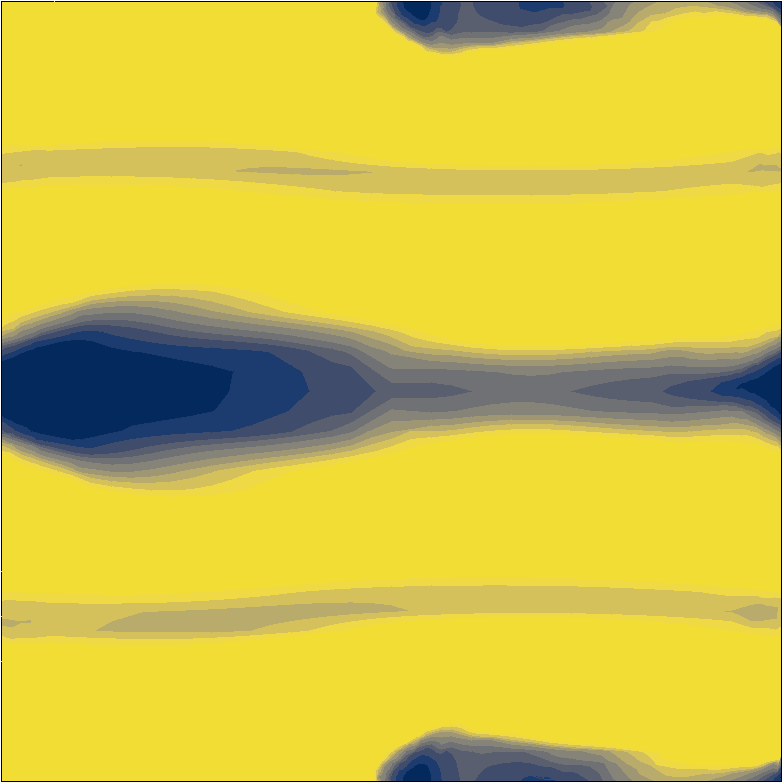
\includegraphics[width=\figninepanelwidth]{image_2/Figure12/DH_2mm_TKE.png} &
        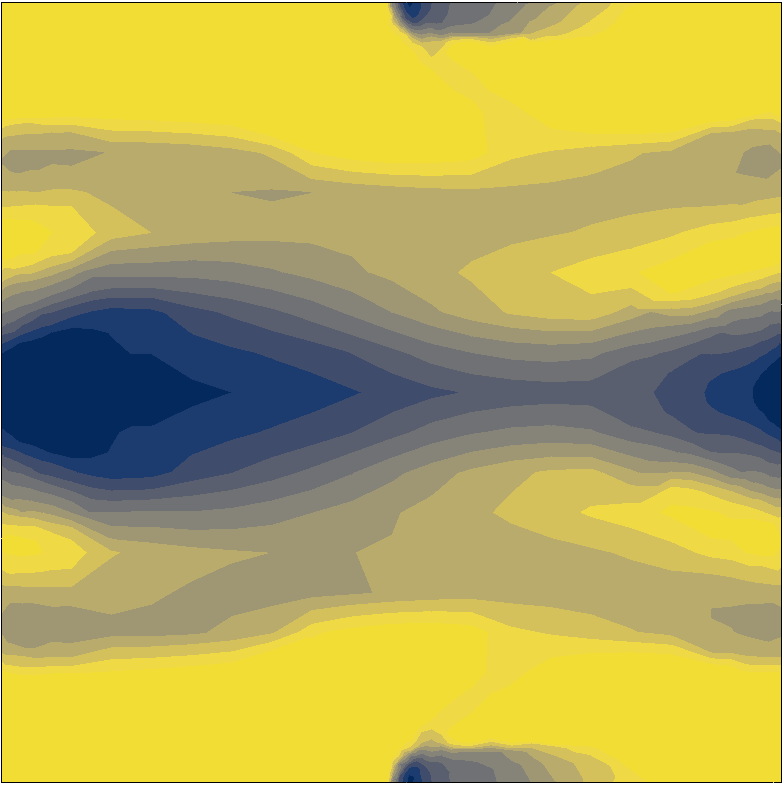
\includegraphics[width=\figninepanelwidth]{image_2/Figure12/DH_3.5mm_TKE.png} &
        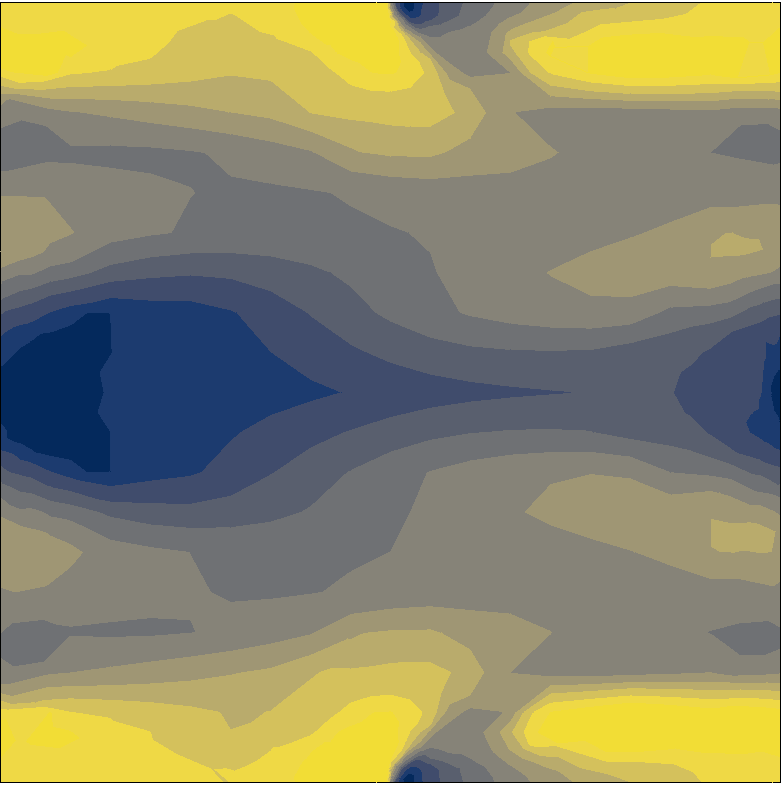
\includegraphics[width=\figninepanelwidth]{image_2/Figure12/DH_5mm_TKE.png} \\[-1pt]
        {\sffamily\fontsize{7.5}{8.5}\selectfont
         \shortstack[l]{$\times 10^{-3}$\\$\mathrm{m^2\,s^{-2}}$}} &
        \figninepanellabel{a}{0.08} &
        \figninepanellabel{b}{0.14} &
        \figninepanellabel{c}{0.20}
    \end{tabular}
    \endgroup
    \caption{TKE distribution of the middle $z$-axis section of DPHE at representative normalized dimple heights ($h_d/l_d=0.08$, $0.14$, and $0.20$).}
    \label{figure9}
\end{figure}
